\documentclass[11pt]{article}

%---------------------------------------------------------------------------------------------------%
%% PACKAGES
%\usepackage{fullpage}
%\usepackage[top=1in, bottom=1in, left=1in, right=1in]{geometry}
\usepackage{graphicx, amsmath, amssymb, amsfonts, mathtools, mathrsfs, color}
\usepackage{comment, enumerate, tabularx}
\usepackage{hyperref, url}
%\usepackage[justification=RaggedRight]{caption}
\usepackage{outlines,enumitem}
\usepackage{wrapfig, todonotes}
\usepackage{titlesec}
\usepackage{fancyhdr}
\usepackage{subcaption}
\usepackage[sort,nocompress]{cite}
%---------------------------------------------------------------------------------------------------%

\addtolength{\oddsidemargin}{-0.75in}
\addtolength{\evensidemargin}{-0.75in}
\addtolength{\textwidth}{1.5in}
\addtolength{\topmargin}{-0.75in}
\addtolength{\textheight}{1.5in}
% For 11pt size


\titleformat*{\section}{\large\bfseries}
\titleformat*{\subsection}{\normalsize\bfseries}

\pagestyle{fancy}
\lhead{\footnotesize Moore and Quaife}
\chead{\footnotesize Erosion, Transport, and  Dispersion in Granular and
Porous Media}
\rhead{\footnotesize \thepage}
\cfoot{}

%---------------------------------------------------------------------------------------------------%
%% LATEX DEFINITIONS
% Basic editing
\newcommand{\nick}[1]{{\color{red}#1}}
\newcommand{\tocite}{{\color{blue}(to cite) }}
\newcommand{\vsp}[1]{\vspace{#1 pc} \noindent}
\newcommand{\np}{\newpage \noindent}
\newcommand{\here}{{\color{blue} here}}
% Basic math, derivatives
\newcommand{\td}[2]{\frac{d #1 }{d #2}}
\newcommand{\ttd}[2]{\frac{d^2 #1 }{{d #2}^2}}
\newcommand{\pd}[2]{ \frac{ \partial #1}{ \partial #2 } }
\newcommand{\ppd}[2]{ \frac{ \partial^2 #1}{ {\partial #2}^2 } }
\newcommand{\mppd}[3]{ \partial_{#2 #3} #1 }
% Basic math, vectors and other
%\newcommand{\bvec}[1]{\ensuremath{\boldsymbol{#1}}}
\newcommand{\bvec}[1]{{\mathbf{#1}}}
\newcommand{\grad}{\nabla}
\newcommand {\Lap} {\grad^2}
\newcommand{\abs}[1]{\left| #1 \right|}
\newcommand{\tavg}[1]{\langle #1 \rangle}
\newcommand{\norm}[1]{ \left\| #1 \right\| }
\newcommand{\ip}[1]{ \langle #1 \rangle }
\newcommand{\eps}{\varepsilon}
% For real and imaginary, could use \Re or \Im, or \mathcal{R}, or \text{Re}
\newcommand{\Pe}{\mathrm{Pe}}

% Outline stuff
\setenumerate[1]{label=\Roman*.}
\setenumerate[2]{label=\Alph*.}
\setenumerate[3]{label=\roman*.}

% Specific
\newcommand{\uu}{\bvec{u}}
\newcommand{\xx}{\bvec{x}}
\newcommand {\qq} {\bvec{q}}
\newcommand{\nn}{{\mathbf{n}}}
\renewcommand{\ss}{{\mathbf{s}}}
\newcommand{\Vn}{V_\nn}
\newcommand{\CE}{C_E}
\newcommand {\ny}{n}
\newcommand {\bdry} {\partial B}
\newcommand{\Diff}{D}
\newcommand{\thL}{$\theta$--$L$}
\newcommand{\bd}{\partial}
\newcommand{\eeta}{\boldsymbol{\eta}}
\newcommand{\rr}{\mathbf{r}}
\newcommand{\ff}{\mathbf{f}}
\newcommand{\yy}{\mathbf{y}}

%---------------------------------------------------------------------------------------------------%


%---------------------------------------------------------------------------------------------------%
%% TITLE
\begin{document}
\begin{center}
{\large \bf Erosion, Transport, and Dispersion in Granular
and Porous Media} 
\\
M.J.N.~Moore and Bryan D.~Quaife
\end{center}
%\title{Project Description --
%Erosion, Transport, Anomalous Diffusion, and Collapse in Granular and Porous Media}

% Original erosion title
%Mathematical models and analysis for erosion and dissolution in porous-media flow}
%\author{}
%\date{}
%\maketitle
%---------------------------------------------------------------------------------------------------%

%---------------------------------------------------------------------------------------------------%
%% INTRODUCTION
\section{Proposed Research} 

\subsection{Introduction and Background} 

Naturally occurring porous and granular materials, such as soil, sand, and clay, play a pivotal role in regulating earth's water resources by filtering contaminants and, over long timescales, supplying fresh water.  Not only is this process essential for human water resources, but also for the ecology of rivers, estuaries, and other natural habitats.  Natural water resources, however, have been placed under enormous pressure by human population growth and associated activities that can compromise the natural filtration cycle, for example expansion of industry, urbanization, pollution, and climate change. See the UN report on water resources for further detail on the threats to water resources~\cite{UNwater}.
% Could also include USGS if needed.

An understanding of these filtration and contamination processes relies on the complex phenomenon of transport in porous media. Further, the action of continually flowing groundwater can alter medium properties through erosive and transportive processes. Thus, it becomes necessary to understand transport through complex media whose properties change {\em dynamically} in response to the intervening fluid flow. These effects are most noticeable during rapid events, like the gravitational collapse of a sinkhole~\cite{sandhu2018fate}, during which medium properties can change dramatically over short timescales. Though less obvious, the accumulation of slower process, such as mechanical or chemical erosion, can also substantially alter medium properties.  

This proposal aims to develop a suite of computational tools geared towards developing a deeper understanding of the physical processes by which groundwater flow can alter porous-media properties and to characterize the associated changes in transport within the evolving medium, for example the anomalous dispersion of tracers. A recognized complexity of naturally occurring media is the heterogeneity and anisotropy of macroscopic properties such as permeability and mechanical strength~\cite{lin2018randomization}. These properties can change over short timescales, for example sinkhole collapse or hydraulic fracturing, or over long timescales, for example the slow erosion or dissolution of solid material. Potential exists for feedback between these timescales: for example the slow wearing process reaching a critical threshold beyond which catastrophic events become more likely.  Physical mechanisms that can alter porous-medium properties include: 
\begin{itemize}[noitemsep]
\item Erosion of solid material due to fluid-mechanical stresses or chemical dissolution.
\item Transport of grains due to intervening fluid flow and due to sedimentation.
\item Compaction of the medium due to overlying loads.
\item Gravitational collapse of a medium due to loads exceeding a threshold.
\end{itemize}
The above are roughly ordered according to timescale, from the slowest acting to the fastest. While many of these mechanisms have been studied individually in various contexts and to varying levels of rigor, very little is known about their combined effect on the dynamic evolution of a porous medium. Since we aim to build a quantitative model from the ground up, we will first focus on the slowest acting mechanisms, as these ultimately set the stage for the more rapid events like sinkhole collapse. 

In particular, we view the accumulated effects of slow processes like erosion and dissolution as instrumental in altering porous-medium properties. First, by deteriorating solid material, erosion alters the size distribution of grains, enabling smaller grains to be sieved through networks of larger ones. A second and more subtle way that erosion can alter medium properties is by changing the {\em shape} distribution of grains. For instance, erosion can carve grains into slender shapes aligned primarily in the direction of the dominant flow, thereby creating {\em anisotropic} characteristics. Likewise, chemical dissolution can carve well-defined conduit paths in karst networks which strongly alter transport properties~\cite{szymczak2009wormhole}.

More generally, the coupling between shape and flow during erosion, dissolution, and related phase-change processes is a topic that has garnered recent interest in the mathematical sciences community~\cite{Ristroph2012, rycroft2016asymmetric, cohen2016erosion, MooreCPAM2017, mitchell2017generalized, Quaife2018, wykes2018self, lachaussee2018competitive, lopez2018cfd, ristroph2018sculpting}.  Erosion-induced shape change has been studied in the high Reynolds number regime, both experimentally~\cite{Ristroph2012, MoorePOF2013} and theoretically~\cite{MoorePOF2013, MooreCPAM2017, hewett2017evolution} and in single~\cite{Ristroph2012, MoorePOF2013, MooreCPAM2017, lachaussee2018competitive} and multiple-body arrangements~\cite{hewett2017evolution}.  Studies on related processes of dissolution~\cite{HuangJFM2015, kondratiuk2015steadily, cohen2016erosion, claudin2017dissolution, wykes2018self, huang2017solute}, melting~\cite{Cummings1999, back2014effect, rycroft2016asymmetric, hewett2017pear, MooreCPAM2017, toppaladoddi2018combined, hewett2019evolution, favier2019rayleigh}, solidification~\cite{Huppert90, Anderson95, Cummings1999, mccue2003extinction}, and deposition~\cite{hewett2018modelling} exhibit intriguing similarities and differences~\cite{MooreCPAM2017}.  These studies reveal a rich set of possible dynamics, from the emergence of universal morphologies that erase details of the initial state and evolve self-similarly in time~\cite{MoorePOF2013, MooreCPAM2017, hewett2017pear}, to fine-scale pattern formation~\cite{cohen2016erosion, claudin2017dissolution, huang2017solute}, to unstable morphologies that can retain or even amplify features present in the initial state~\cite{claudin2017dissolution, wykes2018self}.
	
Only recently have these ideas been extended to the low-Reynolds-number regime that is applicable to porous media~\cite{mitchell2017generalized, Quaife2018}. While the governing fluid-flow equations become linear in this regime, porous-media applications present a host of new challenges, for example:
\begin{itemize}[noitemsep]
\item Porous media typically involves dense packings so that close-range effects and even nearly contacting bodies must be considered.

\item The Stokes limit introduces {\em longer} range effects than the inertial limit does, thus coupling the shape evolution of {\em all} grains and conduits to a higher degree.

\item Somewhat counterintuitively, erosion does not always act to smooth shapes but rather can create sharp features and corners~\cite{Ristroph2012}. These features can be difficult to resolve and, further, can trigger numerical instabilities~\cite{Quaife2018}. Dissolution, meanwhile, can initiate a roughening transition~\cite{claudin2017dissolution}, leading to similar numerical difficulties.

\item Additionally effects, such as sedimentation, transport, and compaction constantly work to reconfigure the medium as its constituents and boundaries degrade.
\end{itemize}
These challenges require innovative computational techniques, some of which have been developed recently~\cite{Quaife2018} and others that await resolution. An ultimate goal of this proposal is to achieve high-fidelity simulations of $\mathcal{O}(100-1000)$ mobile bodies undergoing simultaneous erosion, transport, sedimentation, and compaction, with the computational efficiency required to run large ensembles for statistical analysis. Dynamic erosion of porous media is a highly active area of research, as closely related laboratory experiments on erosion in colloidal systems are already being explored in the Datta Lab at Princeton~\cite{bizmark2019multiscale}. These experiments a great opportunity for comparison against our numerical simulations. Furthermore, we propose performing a set of experiments conducted at the nearby the Geophysical Fluid Dynamics Institute, which would help to guide, calibrate, and validate the computations (see letter of collaboration).


While erosion and dissolution lead to gradual changes in a medium, other events like sinkhole collapse or hydraulic fracturing occur over much shorter timescales.  Most likely, all of the mechanisms listed above---erosion, dissolution, transport, compaction, and gravitational collapse---contribute to sinkhole formation, with the slowest acting mechanisms creating conditions favorable for the final act of gravity. Sinkhole formation has been explored in preliminary experiments conducted at the Geophysical Fluid Dynamics Institute (GFDI) at Florida State University~\cite{tao2014experimental}. These scaled-down experiments offer the ability to probe various mechanisms behind sinkhole formation, for example a difference in hydraulic head between the confined and unconfined aquifers. An ultimate goal of the project proposed here is to merge these two lines of inquiry to gain a deeper understanding of the influence of mechanically or chemically induced erosion on gravitational collapse.  Ultimately, we envision the high-fidelity erosion simulations to inform coarse-grained models for: (i) transport and dispersion; and (ii) dynamic evolution of macroscopic medium properties. These parameterized models could then be combined with well-developed multi-phase models~\cite{Imma2019, eastham2019multiphase} to quantitatively describe and predict sinkhole collapse.


%---------------------------------------------------------------------------------------------------%
\subsection{Governing equations}

We first summarize governing equations underlying the proposed work.
At the finest scale, the fluid flow intervening between individual grains of a porous medium is governed by the incompressible Stokes equations
\begin{equation}
\label{StokesEq}
\begin{split}
\mu \Delta \uu = \grad p,	&\hspace{20pt} \xx \in \Omega, \\
\grad \cdot \uu = 0, 		&\hspace{20pt} \xx \in \Omega,
\end{split}
\end{equation}
where $\uu$ is the velocity field, $p$ the pressure field, and $\mu$ the fluid viscosity. Linear elliptic PDEs, such as the Stokes equations, can be reformulated as a boundary integral equation (BIE).  BIEs have several numerical advantages including a dimension reduction, automatic mass conservation, and high-order accuracy. An equivalent BIE formulation of the Stokes equations in Eq.~\eqref{StokesEq} is
\begin{align}
  \label{eqn:BIE}
  \ff(\xx) = -\frac{1}{2}\eeta(\xx) + \frac{1}{\pi} \int_{\bd\Omega}
    \frac{\rr \cdot \nn}{\rho^2} \frac{\rr \otimes \rr}{\rho^2}
    \eeta(\yy) ds_\yy, \quad \xx \in \bd\Omega
\end{align}
where $\ff$ is a Dirichlet boundary condition, $\rr = \xx - \yy$, $\rho = \|\rr\|$, and $\nn$ is the outward unit normal of $\bd\Omega$.  Once~\eqref{eqn:BIE} is solved for the density function $\eeta$, important quantities such as the velocity, pressure, vorticity, and deformation tensor can be computed in the fluid bulk.  For example, the velocity at $\xx \in \Omega$ is 
\begin{align}
  \uu(\xx) = \frac{1}{\pi} \int_{\bd\Omega}
    \frac{\rr \cdot \nn}{\rho^2} \frac{\rr \otimes \rr}{\rho^2}
    \eeta(\yy) ds_\yy.
\end{align}

Eq.~\eqref{StokesEq} is a microscopic description is required to study the shape evolution of individual grains due to fine-scale erosive effects, either mechanical or chemical. The description, however, becomes impractical when attempting to model seepage in very large porous systems where the microscopic geometry can be exceedingly complex. Instead, one must homogenize over microscopic details to arrive at an approximate description. Leading-order homogenization produces the well-known Darcy system 
\begin{align}
  \label{DarcyEq}
  \qq = - \bvec{K} \grad \phi
\end{align}
where $\qq$ is the {\em specific discharge} or {\em Darcy velocity}, and $\phi = z + p/(\rho g)$ is the hydraulic head, with $\rho$ and $g$ representing the fluid density and gravitational constant respectively.  Above, $\bvec{K}$ is the {\em conductivity}, which is related to the {\em permeability} $\bvec{k}$ through $\bvec{K} = \bvec{k} \rho g/\mu$.  Both the conductivity and permeability are in general tensors, and they reduce to scalars in the case of an isotropic medium. Note that the Darcy velocity is related to the tracer velocity through $\qq = \theta_f \uu$, where $\theta_f$ is porosity (i.e.~fluid volume fraction).  In the case of an isotropic medium, the Kozeny-Carman equation is often used to relate permeability to volume fraction~\cite{bear2013dynamics}
% See Bear Ch. 2.8, pg. 111
\begin{align}
  k = C \frac{\theta_f^3}{(1-\theta_f)^2}.
\end{align}
The macroscopic description offered by Eq.~\eqref{DarcyEq}, although approximate, simplifies analysis tremendously in that individual grains are no longer resolved and thus the domain geometry is generally much simpler.

While the most immediate proposed work on computational methods to simulate erosion will utilize~\eqref{StokesEq}, the later stages of this project will also incorporate~\eqref{DarcyEq}, or closely related variants known as multiphase models~\cite{Imma2019, eastham2019multiphase}, in order to develop coarse-grained descriptions for porous medium evolution and the associated dispersion within. These models will rely on statistical analysis of the data produced by the high-fidelity erosion simulations in order to parameterize the effects of erosion, leading to deterministic or stochastic reduced-order models for porous-medium evolution. 
%and erosion, combined with other external effects such as gravitationally-induced dynamics.  

%---------------------------------------------------------------------------------------------------%
\subsection{Mechanical and chemical erosion of a porous medium}

The first problem discussed here is the erosion of a porous medium, as has been preliminarily investigated in~\cite{Quaife2018}. We will consider erosion induced by either fluid-mechanical forces or by chemical reaction, i.e.~dissolution. In the former case, erosion results from surface shear stress
\begin{align}
\tau = -\left(\nabla \uu + \nabla \uu^T \right)\nn \cdot \ss \, .
\end{align}
where $\nn$ and $\ss$ are the unit normal and tangent vectors on the surface respectively and $\uu$ is the velocity field as computed from the incompressible Stokes equations \eqref{StokesEq}. 
The motion of the interface is proportional to the absolute value of shear
\begin{align}
\Vn = \CE \, \abs{\tau},
\end{align}
In the latter case of chemically-induced erosion, a solute concentration field $C$ undergoes advection and diffusion:
\begin{align}
\label{Ceq}
& \pd{C}{t} + \uu \cdot \grad C = \Diff \Lap C \, ,
\end{align}
Material removal is then governed by Fick's law with interface velocity
\begin{equation}
\label{DissVn}
\Vn = \left. \Diff \pd{C}{\ny} \right. %\right\vert_{\bdry} \, ,
\end{equation}
Both processes have been investigated by the PIs and collaborators in
the context of single bodies in high Reynolds-number
flows~\cite{Ristroph2012, MoorePOF2013, HuangJFM2015, MooreCPAM2017}. In
the low-Reynolds regime of porous-media flow, numerical methods have
been developed by the PIs to simulate shear-induced
erosion~\cite{Quaife2018}. These simulations combine highly accurate
boundary integral methods with stable interface evolution techniques.
The boundary integral solver is accelerated by the fast multipole
method~\cite{gre-rok1987, gre-gre-may1992} to achieve optimal $O(N)$
complexity. Meanwhile, the so-called {\thL} method is used for interface
evolution to prevent distortion and tangling of the interface meshes~\cite{hou1994removing, MoorePOF2013, Quaife2018}.
%A near-term goal is to adapt these methods to handle the case of chemically-induced dissolution.

%\subsubsection{Basic dynamics}

%^^^^^^^^^^^^^^^^^^^^^^^^^^^^^^%
\begin{figure}%[htbp]
\begin{center}
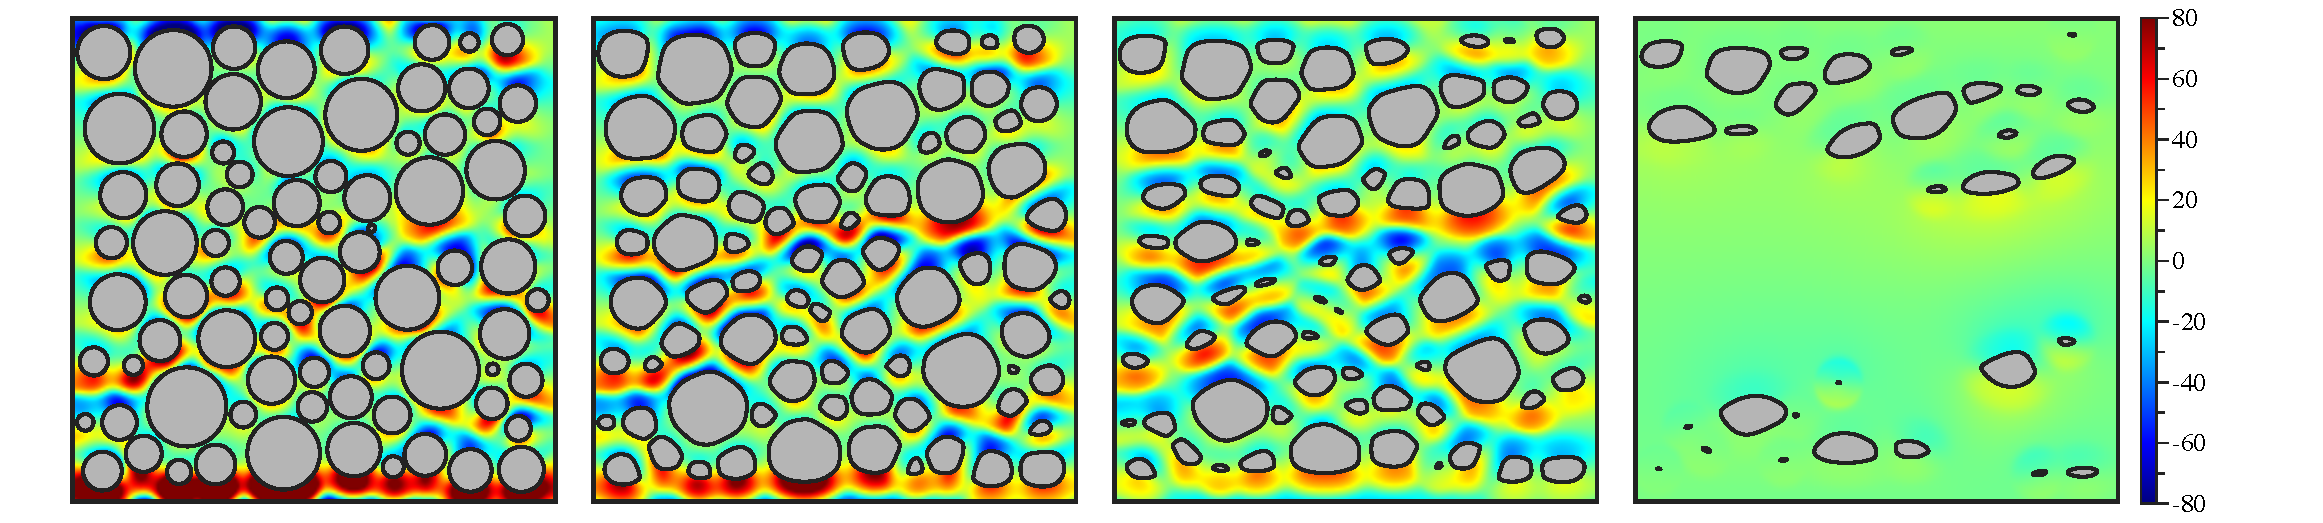
\includegraphics[width = 0.99 \textwidth]{./figs/80circ8vort.pdf}
\caption{\label{fig1} Simulation of 80 bodies eroding in Stokes flow under the action of shear stress. Flow is left to right. Color represents vorticity, which provides a convenient way to visualize local shear rates. 
%Erosion not only diminishes the size of the bodies but also alters their shapes considerably. A few well-defined channels develop in the space between bodies. Several of the bodies vanish in finite time and the simulation continues without interruption.
}
\end{center}
\end{figure}
 %^^^^^^^^^^^^^^^^^^^^^^^^^^^^^^%
 
 Figure \ref{fig1} shows preliminary results of multiple bodies undergoing mechanical erosion in Stokes flow. The figure shows 80 bodies of initially random size and position, undergoing erosion. This figure extends previously reported 50-body simulations to 80 bodies~\cite{Quaife2018} due to a recently developed Barycentric interpolation scheme~\cite{bar2014, bar-wu-vee2015}, which enables closer contact between bodies and thus more bodies.
The color shows the (normalized) vorticity field surrounding the bodies. Vorticity, since it reduces to shear on solid interfaces, provides a convenient way to visualize local erosion rates, as well as the local flow intensity. Observe that erosion not only reduces the size of solid bodies, but also alters their shapes substantially. The bodies tend to become somewhat polygonal: corners develop connected by relatively flat faces. The number of faces does not appear to be easily predicted, but rather depends on the interaction with neighboring bodies as mediated by the Stokes flow. Notice that, as erosion proceeds, relatively straight channels tend to develop between the bodies. Certain channels that are initially larger can transmit more flow, which promotes local erosion rates and further widens these selected channels. In this way, erosion creates a runaway process in which small differences in initial channel size become amplified. The channelization process is made more evident by visualization of the velocity magnitude, as in Fig.~\ref{fig2}.

%^^^^^^^^^^^^^^^^^^^^^^^^^^^^^^%
\begin{figure}%[htbp]
\begin{center}
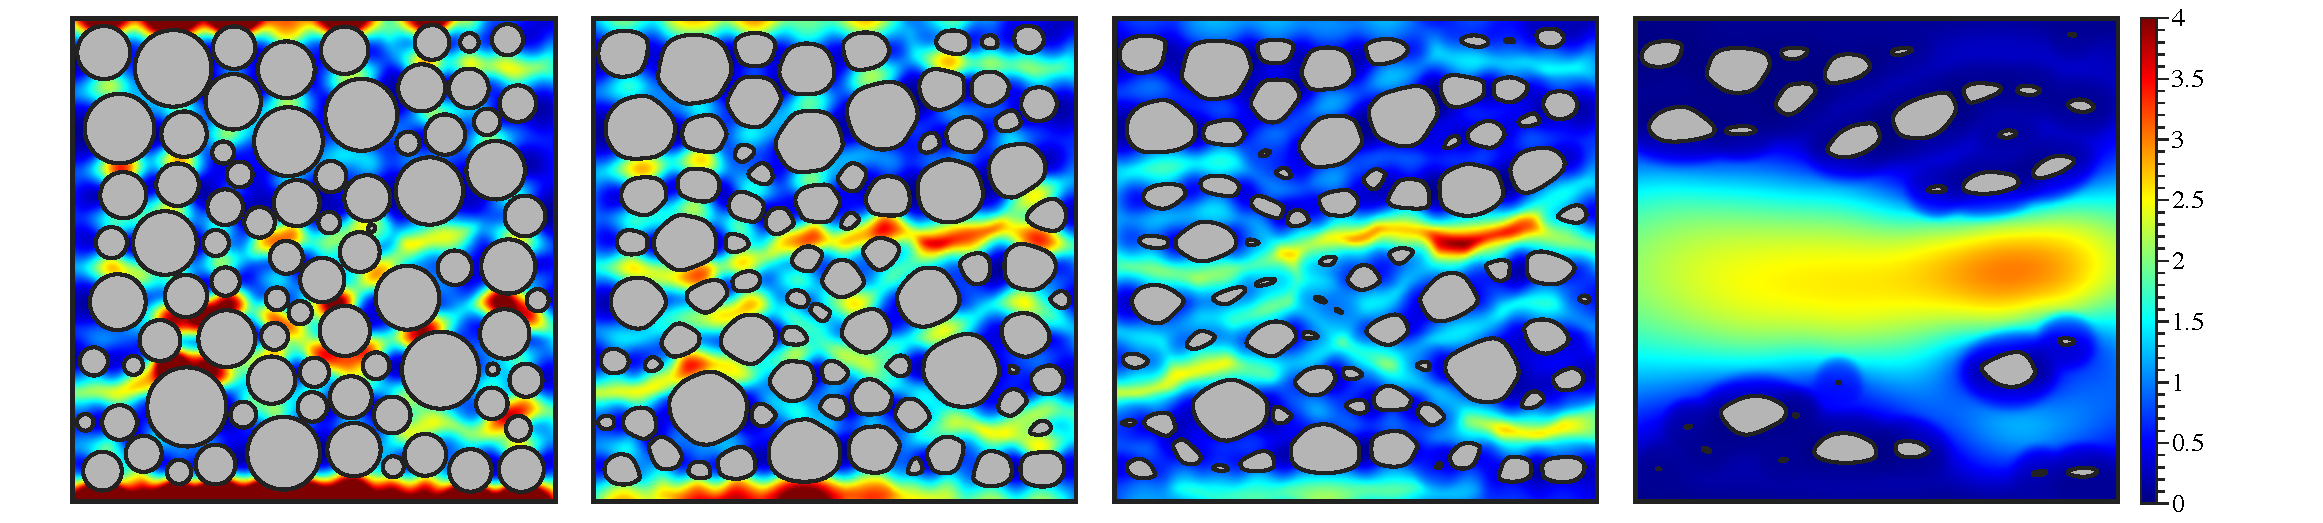
\includegraphics[width = 0.99 \textwidth]{./figs/80circ8vel.pdf}
\caption{\label{fig2} The same simulation as above with velocity magnitude in color. Velocity magnitude highlights the most dominant channels whose growth is reinforced by the shape-flow interaction of erosion.}
\end{center}
\end{figure}
 %^^^^^^^^^^^^^^^^^^^^^^^^^^^^^^%
 
%\subsubsection{Evolution of macroscopic properties}

The creation and reinforcement of channels significantly impacts the macroscopic properties of the porous medium. Fig.~\ref{fig3} shows new, preliminary results on how media properties change in time. First, the left-most plot shows the rate at which the area fraction decreases as the bodies erode. 
%Time is normalized by the value $t_f$ at which all bodies vanish and hence the area fraction is zero. 
Notice that the rate of area reduction does not change significantly during the simulation. The middle plot shows the resistivity, or inverse permeability of the medium. In the simulations, resistivity is calculated by measuring the total flux and the pressure upstream and downstream, then using Darcy's relation \eqref{DarcyEq} to infer the horizontal permeability $k_x$. Naturally, as bodies erode, the resistivity they provide decreases in time. Note that, unlike the area plot, the vertical axis is logarithmic and so the straight line observed at early times indicates that the resistivity decreases exponentially. The much more mild decrease in area fraction is not sufficient to account for this exponential rate, and hence the reshaping process, in particular the formation of channels, plays a pivotal role.

Lastly, the right-most plot of Fig.~\ref{fig3} shows the anisotropy, which is calculated as the ratio of the vertical resistivity to the horizontal resistivity, see Eq.~\eqref{DarcyEq}. The vertical resistivity is computed by rotating the configuration of bodies by 90 degrees. This plot shows the anisotropy to initial increase with time. Thus, the initially isotropic state becomes erased as bodies streamline and form primarily horizontal channels. Remarkably, the medium reaches an anisotropy of over 10, meaning that erosion can lead to a configuration that resists flow 10 times more in the vertically than horizontally.

%^^^^^^^^^^^^^^^^^^^^^^^^^^^^^^%
\begin{figure}%[htbp]
\begin{center}
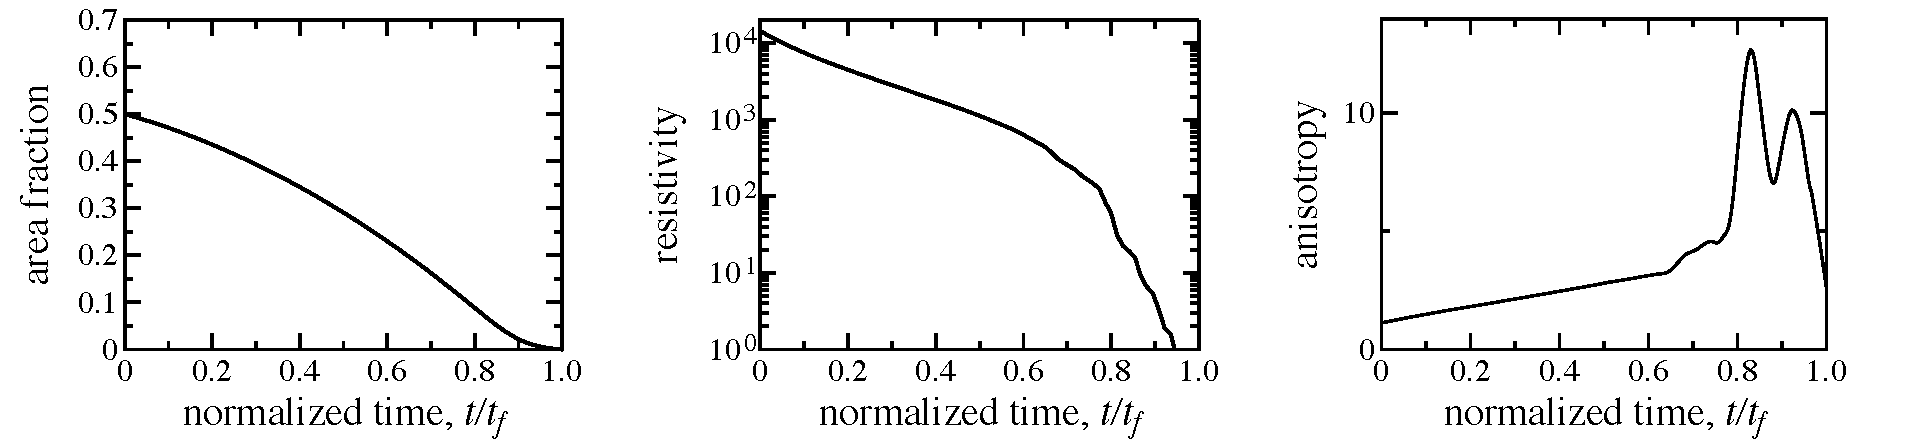
\includegraphics[width = 0.99 \textwidth]{./figs/fig3.pdf}
\caption{\label{fig3} Left: the area fraction of solid bodies versus time. Time is normalized by the vanishing time $t_f$. Middle: the resistivity of the porous matrix decrease much more rapidly than area fraction, indicating the reshaping process to be essential. Right: the anisotropy (ratio of vertical to horizontal resistivity) as it varies in time. Erosion can create a highly anisotropic medium.
}
\end{center}
\end{figure}
 %^^^^^^^^^^^^^^^^^^^^^^^^^^^^^^%

%\subsubsection{Immediate goals of proposed work}

An immediate goal of the proposed work is extend the range of physical effects captured in these simulations. A particular challenge of a BIE formulation is developing quadrature for nearly-singular integrands that arise when bodies are close. To address this problem, we have very recently extended a Barycentric quadrature~\cite{bar2014, bar-wu-vee2015} and have successfully simulated erosion with grains that are initially separated by 1\% of an arclength spacing~\cite{chi-moo-qua2019}. This quadrature approach has the advantage that it is a non-intrusive modification of the trapezoid rule, allowing us to achieve an error bound that independent of the grain configuration. Near-term plans are to include flow transport and gravitational sedimentation of the eroding grains. For this extension, contact forces between bodies must be included to eliminate unphysical contact that is inevitable due to discretization errors. 

Though conceptually straightforward, implementing contact forces in multibody fluid-structure simulations is far from simple in practice, with several competing possible strategies that are a topic of current research.  One approach is to use introduce a potential with short-range repulsion, but such methods often introduce stiffness. Alternatively, a space-time interference volume can guarantee a minimum separation between grains.  In a fluid context, this method was first introduced by Lu et al.~\cite{lu-rah-zor2017}, and extended to allow for much smaller separation distances of rigid bodies by the PI's previous graduate student~\cite{bys-sha-qua2019}. One Ph.D.~student, who will be jointly supervised by both PIs, will simulate sedimentation of eroding bodies by developing algorithms that resolve quadrature error and contact.

Next, we plan to extend the simulation framework to handle chemical dissolution of solid bodies via physical laws~\eqref{Ceq}--\eqref{DissVn}. For this goal, much of the computational infrastructure, such as the boundary-integral solver for the Stokes equations, is already in place, but the coupling to the advection-diffusion equations~\eqref{Ceq} and interface law~\eqref{DissVn} need to be implemented.  We proposed to solve the advection diffusion equation~\eqref{Ceq} by first using Strang splitting~\cite{str1968} to decompose the PDE into linear advection and diffusion.  The advection equation will be solved with a semi-Lagrangian method~\cite{rob1981} so that it can be solved on an Eulerian grid without a restrictive CFL condition. PI Quaife has experience with using semi-Lagrangian methods for another type of complex viscous flow~\cite{kab-qua-bir2017}.  The diffusion equation is more challenging to accurately solve in the complex porous geometries.  Two approaches include a memory-intensive space-time heat kernel~\cite{bar-eps-gre-jia-wan2019, jia-gre-wan2015, li-gre2009}, and Rothe's method coupled with a Yukawa equation solver~\cite{kro-qua2010, cau-cho-chr-sea2016}. A particular challenge of the latter method is extending functions from the complex geometry and into a regular geometry, such as a square, so that a high-order volume integral or Fourier method can be applied, and some groups have recently developed new techniques to form such an extension~\cite{fry-kro-tor2019, fry-leh-tor2019}. Alternatively, we propose to use a Laplace Transform to solve the diffusion equation
\begin{alignat}{3}
  \pd{c}{t} &= \frac{1}{\Pe} \Delta c, \quad &&\xx \in \Omega, \: t>0.
\end{alignat}
Applying the Laplace transform, $C(\xx,s) = \mathcal{L}[c](\xx,t)$ satisfies
\begin{align}
  sC(\xx,s) - \frac{1}{\Pe}\Delta C(\xx,s) = c_0(\xx), 
    \quad \xx \in \Omega,
  \label{eqn:DiffusionLaplace}
\end{align}
where $c_0(\xx)$ is the initial concentration. This PDE will be solved with high-order accuracy and efficiently by using fast-multipole-accelerated integral equation methods of the Yukawa equation~\cite{kro-qua2011}, and the concentration will be recovered with an inverse Laplace transform~\cite{jos-war2006}.  
Once a high-order advection-diffusion solver is in place, by combining it with our integral equation formulation for the Stokes equation and the shear stress, simulations of simultaneous erosion and dissolution, while also including transport and sedimentation, would finally become possible. Such a framework could accurately simulate the geophysically relevant scenario of karst conduits with embedded granular media. The gradual changes in the medium and karst boundaries due to erosion and dissolution could create conditions favorable for mechanical failure or collapse of the structure, for example sinkholes.

 
%---------------------------------------------------------------------------------------------------%
\subsection{Transport through eroded media}

\begin{wrapfigure}[]{r}{0.3\textwidth}
  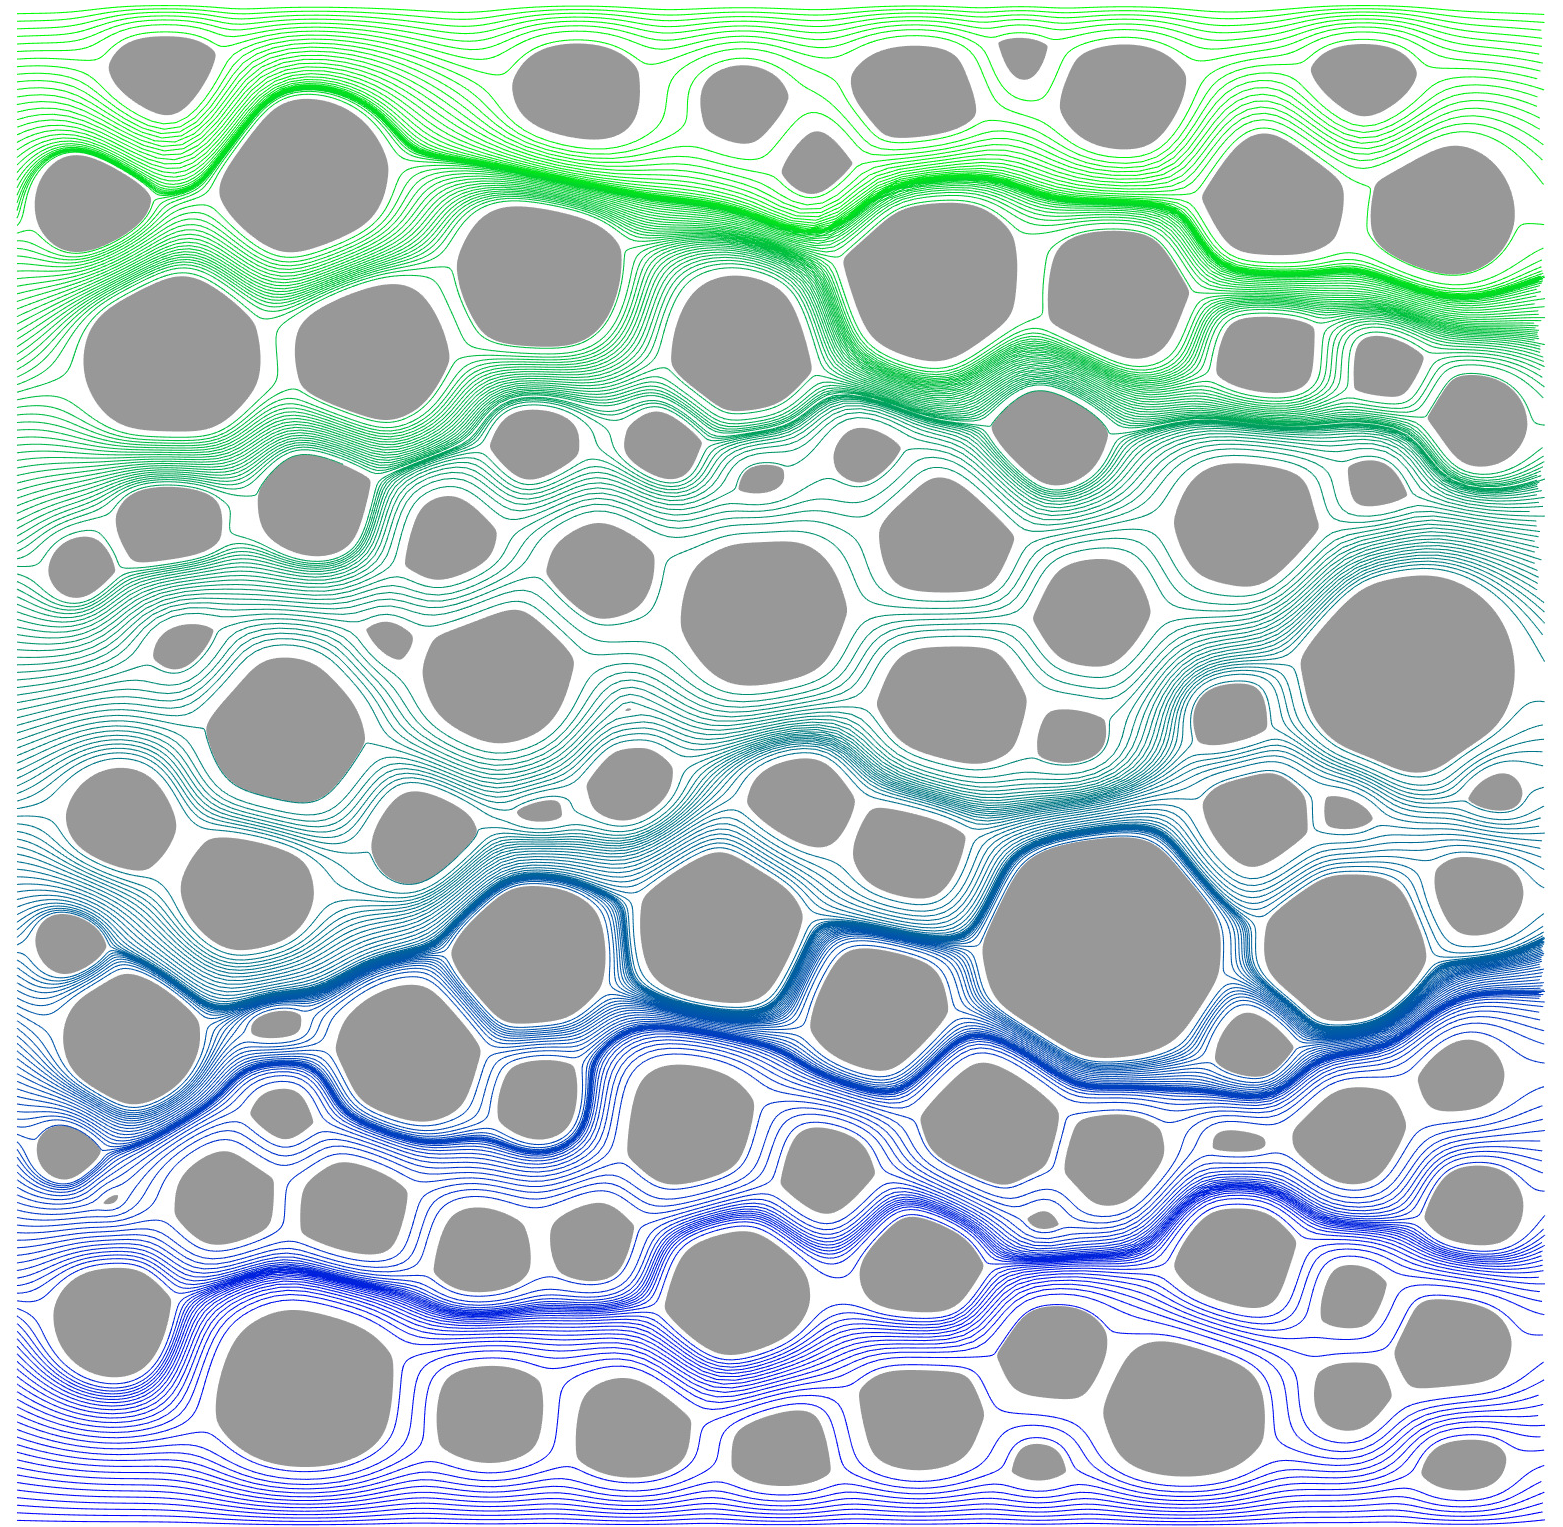
\includegraphics[width=0.3\textwidth]{figs/100b_t100tracer}
  \caption{\label{fig:100tracers} A visualization of the streamlines
  with 200 tracers passing through an eroded geometry with a porosity of
  0.63. The tracers are initialized at the left end of the channel and
  the flow is driven by a pressure difference from left to right.}
\end{wrapfigure}

Transport through eroded media is a direct consequence of the pore structure. Qualitative properties of an eroded media, such as channels of high porosity, can be modest in volume fraction, but can be responsible for a large portion of the flux~\cite{Quaife2018}.  To increase understanding of flow through eroded media, we will simulate and statistically analyze transport through eroded geometries.

In an eroded geometry $\Omega$, the dimensionless
concentration $c$ is governed by
\begin{align}
  \pd{c}{t} + \uu \cdot \nabla c = \frac{1}{\Pe} \Delta c, 
  \label{eqn:advectionDiffusion}
\end{align}
where $\Pe$ is the dimensionless Peclet number. Here we assume that the
concentration $c$ is affected by the eroded geometry, but the geometry
is not altered further by the concentration. In the infinite Peclet
number limit, the concentration is governed by pure advection and the
characteristics of the concentration field are identical to the
streamlines (Figure~\ref{fig:100tracers}).

The $j^{th}$ trajectory, or characteristic, is governed by $\dot{\ss}_j(t) = \uu(\ss_j(t))$. Once these trajectories are computed, using for example a high-order Runge-Kutta method, a statistical analysis can be used to describe the transport. Two of the most important measurements are the tortuosity and the anomalous dispersion, both which are defined in terms of the length of the trajectories \begin{align}
  \lambda_j(t) = \int_{0}^{t} \|\ss'(t')\| dt'.
\end{align}
Upon computing $N_p$ trajectories, the tortuosity is the dimensionless number
\begin{align}
  T = \frac{1}{d} \left(\int_{S} u_1(x_0,y_0)\lambda(y_0) dy_0\, \right)
  \Bigg/ \left(\int_S u_1(x_0,y_0)\, dy_0 \right),
\end{align}
where $S$ is the vertical cross-section at $x=x_0$, $d$ is its length,
$u_1$ is the horizontal velocity, and $\lambda(y_0)$ is the length of
the trajectory starting at $(x_0,y_0)$ and ending at a vertical
cross-section at the other end of the channel. Relationships between the
tortuosity and porosity of a geometry have been developed by other
groups~\cite{kop-kat-tim1996, dud-koz-mat2011, mat-kha-koz2008}, and
preliminary results indicate that such models might be appropriate for
geometries whose porosity is increasing under the process of erosion
(Figure~\ref{fig:100tortuosity}(a)). However, preliminary results also
indicate that erosion can increase the amount of tortuosity as is
evident towards the at the towards the end of the erosion process in
Figure~\ref{fig:100tortuosity}(a). Moreover, we have observed a
significant increase in the tortuosity at small porosities
(Figure~\ref{fig:100tortuosity}(b)).

\begin{figure}[htp]
  \begin{center}
  \begin{subfigure}[b]{0.45\textwidth}
  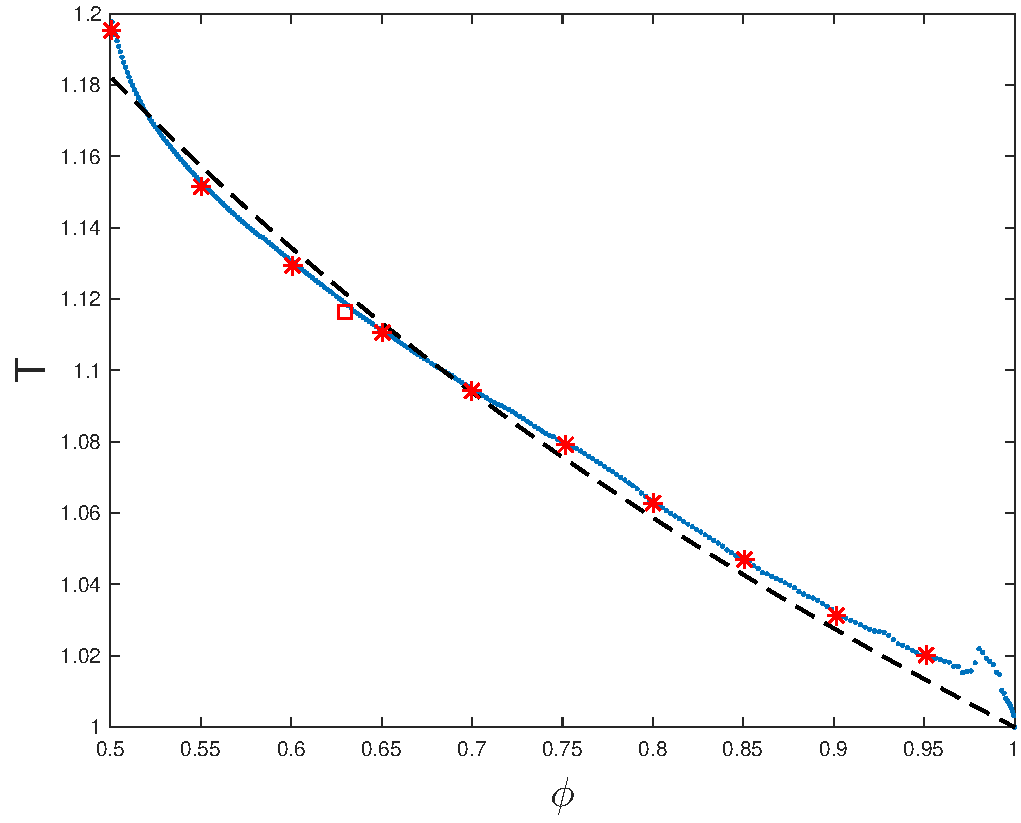
\includegraphics[width=\textwidth]{figs/tort_eulerian100}
  \caption{100 eroding bodies}
  \end{subfigure}
  \begin{subfigure}[b]{0.45\textwidth}
  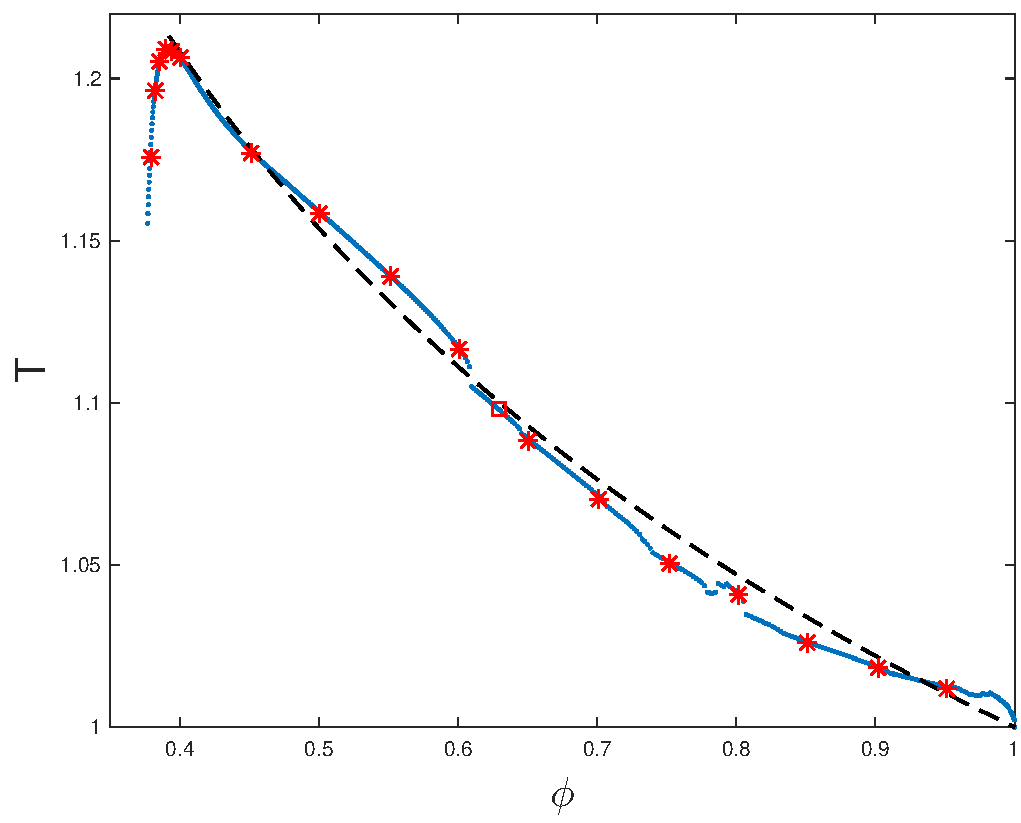
\includegraphics[width=\textwidth]{figs/tort_eulerian20}
  \caption{20 eroding bodies}
  \end{subfigure}
  \end{center}
  \caption{\label{fig:100tortuosity} The tortuosity of two different eroding geometries. The tortuosity can be computed using two different formulas (red vs.~blue marks). In the left plot, the red square is the tortuosity of the geometry in Figure~\ref{fig:100tracers}. In both cases, there is qualitative agreement between our numerical simulations and a power-law model (black dashed line)~\cite{mat-kha-koz2008}.}
\end{figure}

While the tortuosity characterizes the amount of winding of streamlines, the dispersion characterizes the spreading of the trajectories.  Dispersion can be described using the first- and second-ensemble moments of the trajectories
\begin{align}
  \langle \lambda \rangle (t) = \frac{1}{N_p} \sum_{j=1}^{N_p}
    \lambda_j(t), \quad \sigma_\lambda^{2}(t) = \frac{1}{N_p}
    \sum_{j=1}^{N_p} (\lambda_j(t) - \langle \lambda \rangle(t))^2
\end{align}
Then, the standard deviation $\sigma_\lambda$ characterizes the dispersion, and long-time behavior typically results in a power-law scaling $\sigma_\lambda \sim t^{\alpha}$. The power $\alpha$, which quantifies the long-time spreading, is $1$ in a ballistic regime which occurs at early times when the trajectories have not explored much of the porous geometry. However, once the trajectories have traversed a few grains, dispersion in porous media is often super-dispersive with $\alpha \in (0.5,1)$~\cite{dea-leb-den-tar-bol-dav2013}. In Figure~\ref{fig:100dispersion}, we investigate spreading at several different porosities of a porous geometry that is initialized with 100 grains.
\begin{wrapfigure}[22]{r}{0.4\textwidth}
  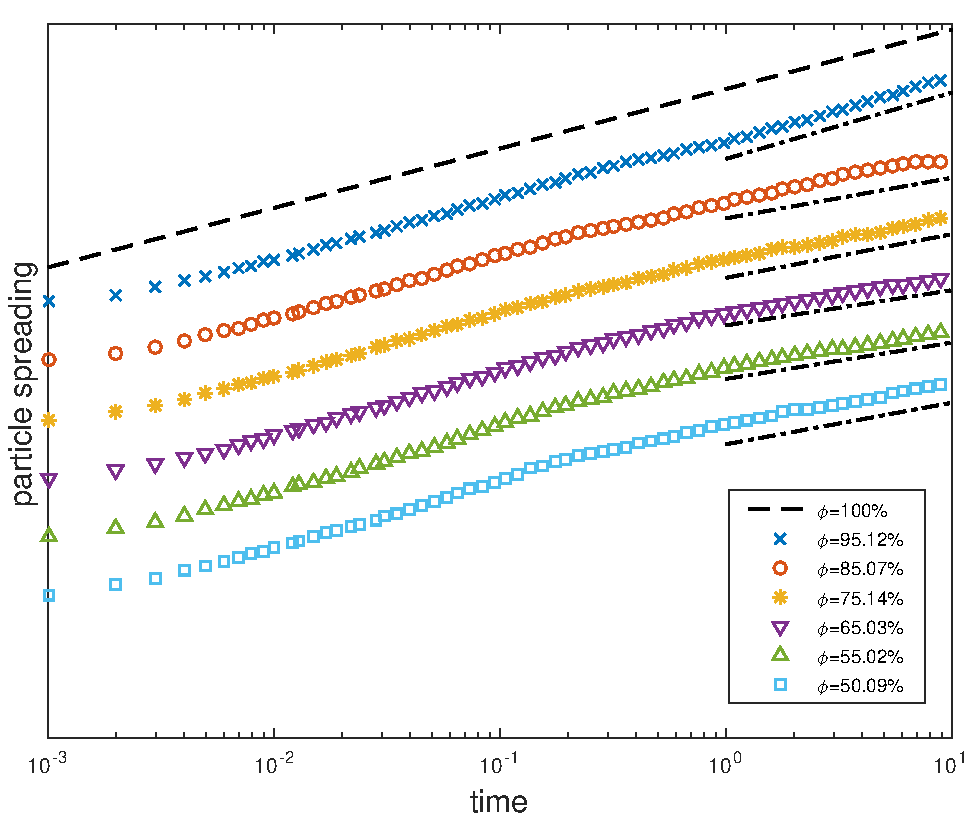
\includegraphics[width=0.4\textwidth]{figs/100b_second_moment_long_ref}
  \caption{\label{fig:100dispersion} The particle spreading,
  characterized with the standard deviation $\sigma_\lambda(t)$ at 6
  different porosities. At early times, the line of slope 1 (black
  curve) indicates a ballistic motion. At later times, the
  dispersion becomes super-dispersive at a rate indicated by the slope
  of the black dashed-dotted line.}
\end{wrapfigure}

The rate of dispersion is known to be directly related to the pore size
distribution~\cite{dea-qua-bir-jua2018}. Therefore, there is a need to
understand how erosion affects the pore size distribution. In
preliminary work~\cite{chi-moo-qua2019}, we define pore sizes between grains that share an edge of a Delanuay triangulation with vertices at the grain centers (Figure~\ref{fig:Eroding100gap_mean_var}(a)). In Figures~\ref{fig:Eroding100gap_mean_var}(a) and~\ref{fig:Eroding100gap_mean_var}(b), we plot the mean and variance of the pore sizes as a function of porosity. To better understand how erosion affects the anomalous dispersion, we propose to investigate how the pores grow with erosion. We will start with the notion of a {\em porelet} which is an individual Hagen-Poiseuille flow in each of the individual pores~\cite{dea-qua-bir-jua2018}. By computing the strength of the individual Hagen-Poiseuille flows, the shear rate can be computed, and thus the rate of erosion can be computed. 

We have performed a carefully chosen simulation to better understand the
effect of erosion on the pore size. We start with a single grain inside
the channel that is sufficiently large that the spacing between the
initial grain and the channel walls, which is 2 units wide), is
$10^{-3}$. Since we use a Barycentric quadrature rule, we are able to
stably simulate erosion with only 512 points on the eroding body which
corresponds to an arclength spacing 12 times larger than the original
separation distance---to achieve a comparable accuracy with the spectral
trapezoid rule, 60 times as many discretization points would be
required. In Figure~\ref{fig:porelets}(a), different shades of grey
correspond to the configuration of the eroding grain at five equally
spaced time steps. At three of the time steps, we plot the velocity
between the grain and the solid wall (black line). At all three
configurations, the flow is nearly parabolic indicating that  porelet
model~\cite{dea-qua-bir-jua2018} is appropriate. After performing a
thorough analysis of the pore size growth in this simple configuration,
we will develop a more complete model for networks of pores that are
prevalent in porous media.


\begin{figure}[htp]
\begin{subfigure}[b]{0.33\textwidth}
  \includegraphics*[height=0.8\linewidth]{figs/triangulation_100b100.pdf}
\caption{}
\end{subfigure}
\begin{subfigure}[b]{0.33\textwidth}
  \includegraphics*[height = 0.8\linewidth]{figs/gap_mean}
\caption{}
\end{subfigure}
\begin{subfigure}[b]{0.33\textwidth}
  \includegraphics*[height=0.8\linewidth]{figs/gap_variance}
\caption{}
\end{subfigure}
  \caption{\label{fig:Eroding100gap_mean_var} (a) The pore sizes are
  defined in terms of a Delanuay triangulation. The effect of erosion on
  (b) the mean and (c) the variance of the pore sizes. The geometry
  initially contains 100 eroding bodies.}
\end{figure}

We propose to extend our preliminary results by considering
concentrations with finite Peclet numbers. We will deploy the same
numerical methods to simulate dissolution and melting to study a
concentration that is being transported through a eroded porous
geometry. Again, this will encompass Strang splitting~\cite{str1968}, a
semi-Lagrangian advection solver~\cite{rob1981}, and a diffusion solver
that solves an $s$-dependent Yukawa equation, where $s$ is the Laplace
transform variable~\eqref{eqn:DiffusionLaplace}.

\begin{figure}[htp]
  \centering
  \begin{subfigure}[b]{0.47\textwidth}
  \begin{center}
  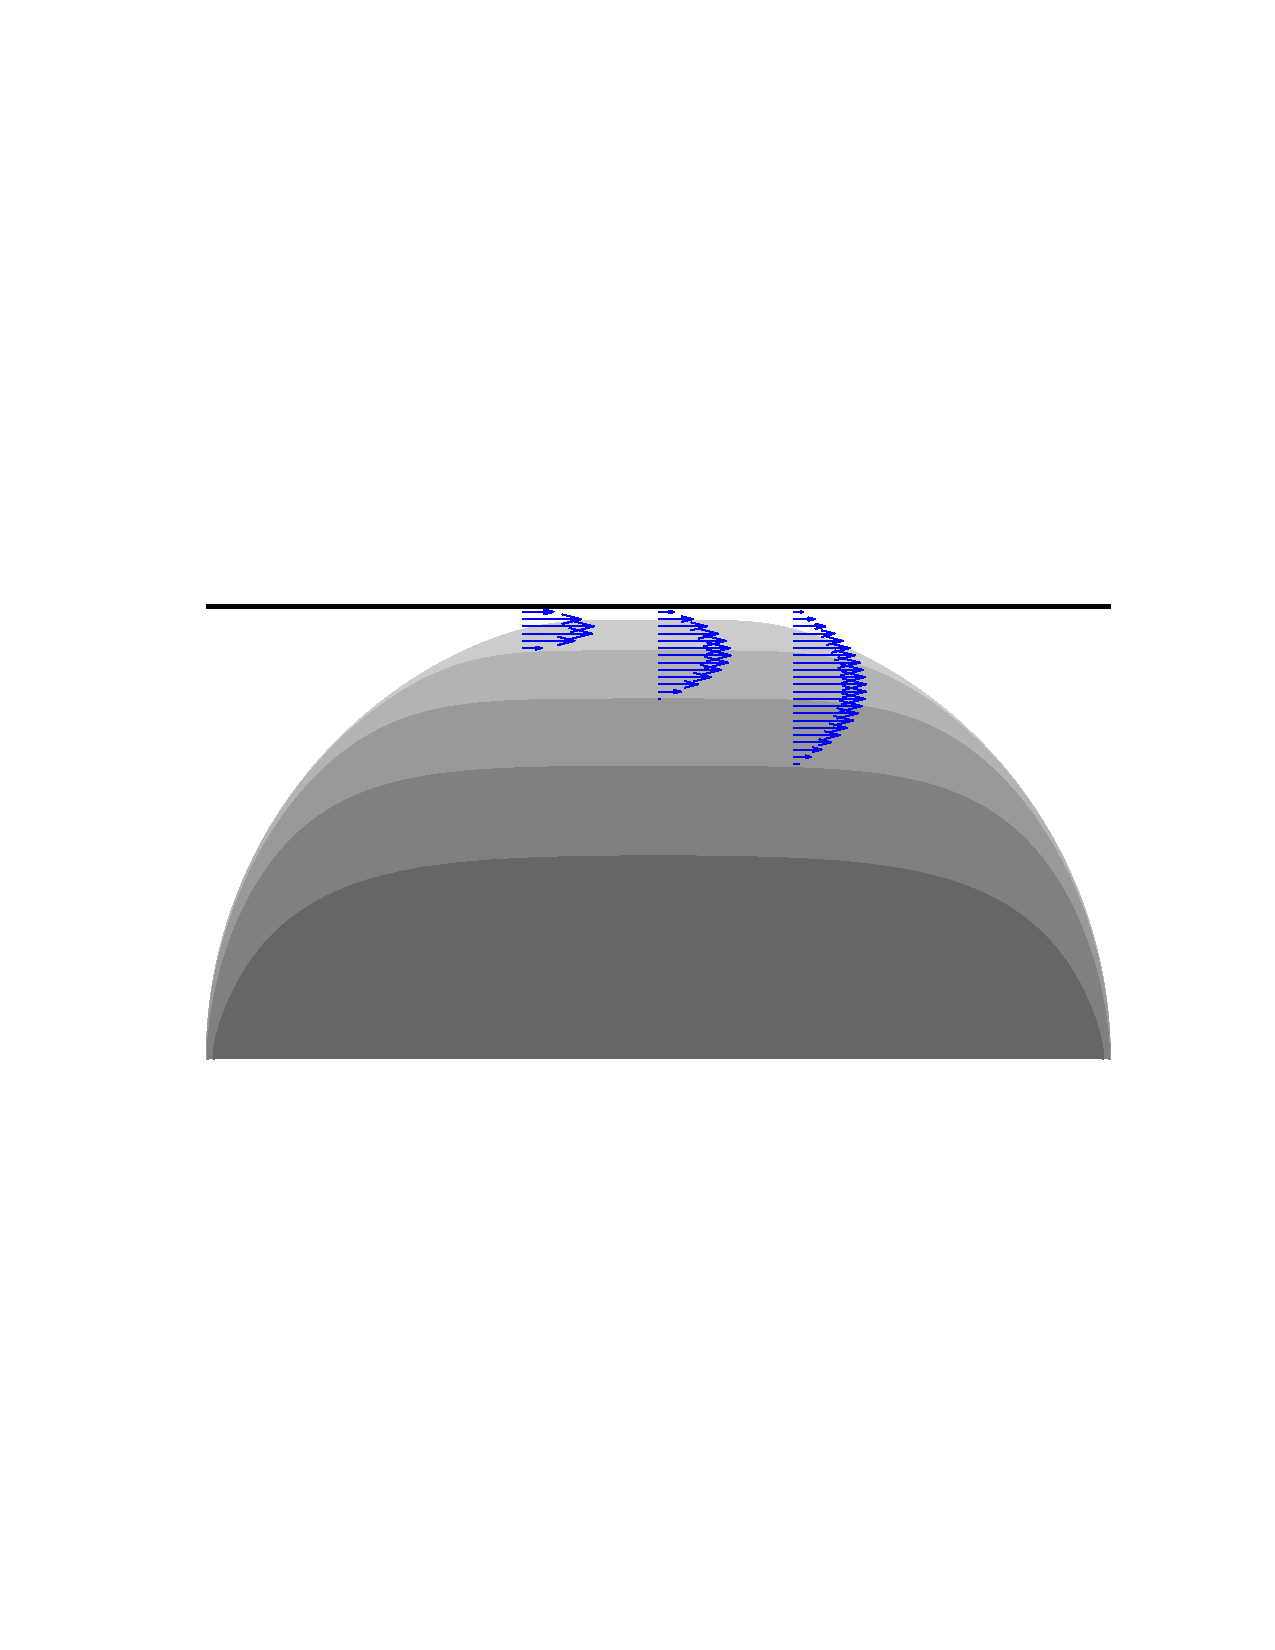
\includegraphics[height=0.55\textwidth]{figs/porelets_geom}
  \end{center}
  \caption{}
  \end{subfigure}
  \begin{subfigure}[b]{0.47\textwidth}
  \begin{center}
  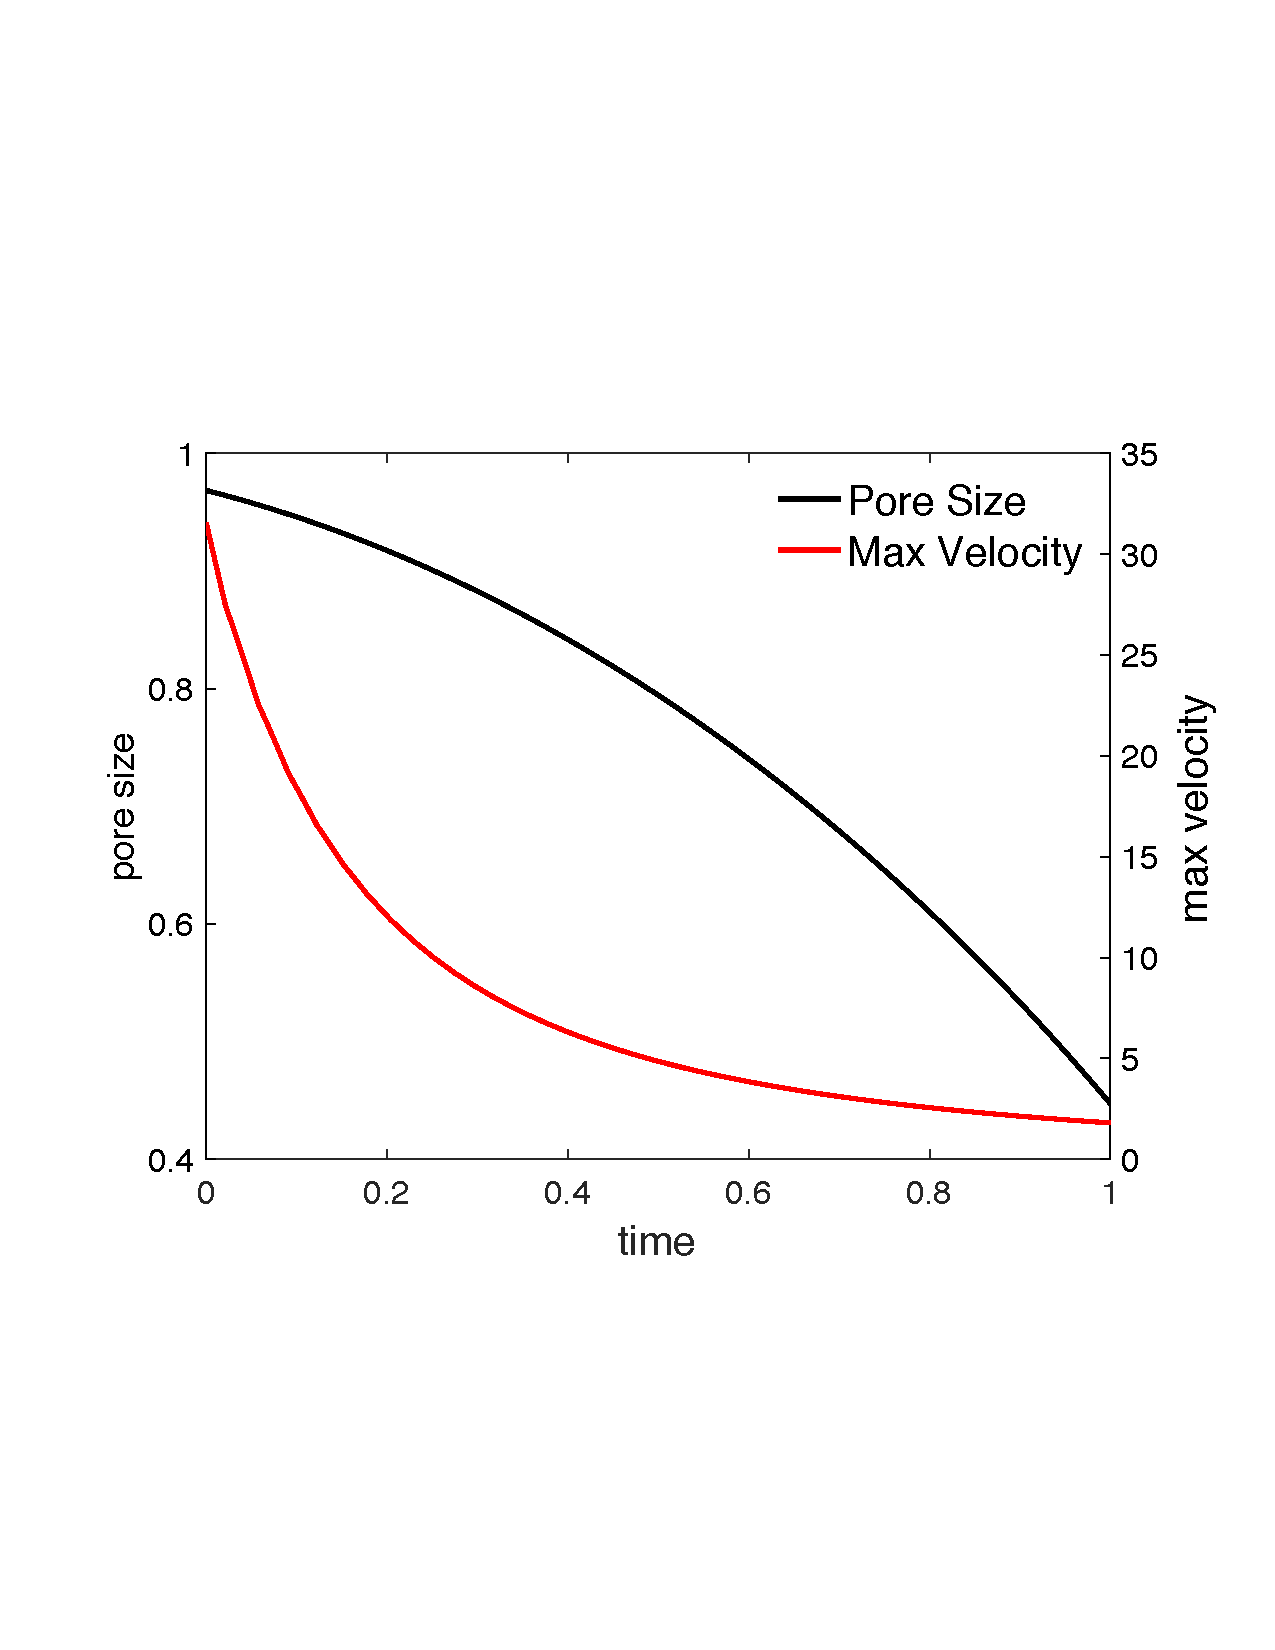
\includegraphics[height=0.55\textwidth]{figs/porelets_size}
  \end{center}
  \caption{}
  \end{subfigure}
  \caption{\label{fig:porelets} (a) An eroding body at five equally time steps in $[0,1]$. The far field condition is a constant pressure drop in a channel three times as wide as the eroding grain.  At the three intermediate time steps, the velocity field in the field, which is nearly parabolic, is included. (b) The pore size (black) and maximum velocity in the pore (red) as a function of time.  As the channel opens, the flow rate increases to maintain a constant pressure drop, and this increases the rate of erosion.} 
\end{figure}


%---------------------------------------------------------------------------------------------------%
% SINKHOLES AND MOBILE BODIES
%---------------------------------------------------------------------------------------------------%

\subsection{Mobile grain simulations and sinkhole formation}

% PREVIOUS PARAGRAPH
%Near-term plans are to include flow transport and gravitational sedimentation of the particles. For this extension, contact forces between bodies must be included. Though conceptually straightforward, implementing contact forces in multibody fluid-structure simulations is far from simple in practice, with several competing possible strategies that are a topic of current research  {\color{blue} cite}. We plan to implement contact forces with {\color{blue} stuff}. This goal will form the PhD dissertation of a graduate student who will be supervised by myself and Prof.~Bryan Quaife (FSU Scientific Computing).

One central goal of this proposal is to enable the free motion of grains during the erosion processes. As mentioned earlier, this goal requires resolving contact forces between bodies, as well as the incorporation of the external buoyancy forces. Once this goal is achieved, it will be possible to simulate a complex porous-medium of arbitrarily sized and shaped grains undergoing the simultaneous action of mechanical-or-chemical erosion and transport due to the combined effects of seepage, contact, and buoyancy forces. These computations will thus simulate, with high-fidelity, the multi-physics of realistic porous-medium dynamics, albeit in a scaled down context. Ultimately, such simulations could be used to build an understanding of medium reconfiguration events, such as sinkhole collapse or conduit formation in karst networks.

In very preliminary work, PI Moore has been running simplified simulations with a current graduate student. These preliminary simulations are based on a hybrid continuum-discrete model for the permeability field and grain particle field respectively. They utilize the homogenized description of the flow field in~\eqref{DarcyEq} and incorporate the physical effects of:
\begin{itemize}[noitemsep]
\item Transport of grains due to seepage force from the surrounding fluid flow.
\item Gravitational sedimentation of grains.
\item Feedback of grain-distribution onto permeability field.
\item Contact and cohesive forces between grains.
\end{itemize}
Preliminary investigation suggests that this last mechanisms of cohesion is essential to model sinkhole collapse in the system.

These simulation have not yet begun to incorporate the slow-acting effects of mechanical and chemical erosion, and the associated gradual changes in medium properties. A grand goal of this proposal would be to merge the two lines of inquiry to develop a sound theoretical framework for porous-medium dynamics robust enough to capture both short-term events, such as sinkhole collapse, and long-term changes in the medium. The greatest challenge faced is the disparate temporal and spatial scales that must be considered. Our proposed strategy is to use the high-fidelity erosion simulations to parametrize the effect of erosion on medium properties.

More specifically, we plan to run large batches of the high-fidelity boundary-integral-equation-based numerical simulations of erosion and then leverage rapid advances in the field of machine learning and deep-neural networks to develop reduced models that parametrize the effects of erosion on the evolution of macroscopic medium properties and the flow.  The output of the high-fidelity simulations of the grain configuration can be transformed into essentially an image format, enabling us to use cutting-edge advancements on deep neural-networks for image analysis~\cite{pelt2018mixed}. Some important advantages of referenced work are the use of dilated convolutions in a deeply connected network, which first mixes scales and second reduces the number of super-parameters present and thus largely averts the risk of overfitting data. Additionally, high-fidelity flow conditions can be used to train a neural network, and this has been successfully used by others to predict, as one example, an anisotropy tensor~\cite{ling2016reynolds}.  Both PIs will supervise a graduate student who will design and implement the deep-neural network for learning the essence of the high-fidelity simulations. Once the essential features are learned, they will be incorporated into reduced-order models that utilize the multiphase framework to enable more efficient and larger scale coarse-grained simulations of dynamic erosion.

As mentioned previously, researchers at FSU's Geophysical Fluid Dynamics Institute (GFDI) have investigated the mechanisms behind sinkhole formation with a series of scaled-down laboratory experiments~\cite{tao2014experimental}. First, already existing data from these experiments offers a testbed for comparison against our newly developed simulations. Furthermore, we propose to run a set of new experiments at the facilities offered by GFDI, spearheaded by an undergraduate student in close collaboration with the graduate students, PIs, and an experimentalist at GFDI. These new experiments will more deeply probe the mechanisms underlying sinkhole formation with the special design goal of comparison against the numerical simulations. These experiments will be used to calibrate and validate our computations.


%---------------------------------------------------------------------------------------------------%
%%%%  SECTION: Education and outreach
%---------------------------------------------------------------------------------------------------%
\section{Broader impacts of the proposed work}

The proposed research could lead to a range of societal benefits, including better management of water resources, accurate prediction of contaminant transport, and an understanding of the long-term effects of human activities, such as hydraulic fracturing or groundwater pumping, on porous media and water resources. In such scenarios, the slow timescales of mechanical and chemical erosion are coupled to the faster timescales of human-induced changes and gravitational collapse. Currently, the relationship between these scales is poorly understood. The high-fidelity, efficient computational methods proposed here will enable a deeper understanding of these processes, which is the first step towards developing effective strategies for managing water resources and mitigating catastrophic events such as contamination or structural collapse. For example, the insights gained here could potentially help identify locations in natural aquifers vulnerable to contamination and/or collapse.

In addition to these societal impacts, the work proposed here will spur the training of mathematicians and computational scientists in fundamentally cross-disciplinary research of great societal importance. Further, the PIs will engage in educational and outreach activities to impact future generations of mathematical scientists, with particular focus on women and underrepresented minorities (URM). Both PIs are already actively involved in graduate and undergraduate research, as well as outreach to K-12 students. Further, we have successfully recruited women and underrepresented minorities in undergraduate, graduate, and postdoctoral research.  

\subsection{Graduate research}
An important benefit of the research proposed here is the potential to immerse graduate students in fundamentally {\em cross-disciplinary} research. This proposal involves a confluence of disciplines, most centrally computational mathematics, but also geophysics, reduced-physical modeling, hydrology, and environmental science.  Exposure to a range of disciplines is, in the view of the PIs, an invaluable opportunity for young scientists.

Naturally, the research proposed here will form the foundation for the
PhD dissertations of the graduate students involved. Beyond this, the
students will engage in publishing articles in peer-reviewed journals of
high quality and attending national and international conferences where
they will present their work and network with experts in the field. The
PIs will closely mentor the graduate students to ensure their continued
development, not only intellectually, but also in the `soft' skills of
communication, promotion, and networking. Having both PIs Moore and
Quaife involved in the training of each graduate student is especially
valuable for offering multiple perspectives on these issues. The PIs
will make special efforts to recruit women and underrepresented
minorities as the graduate students funded by this project. Both PIs
have already had success recruiting women in these roles, as the first
graduate student to receive her PhD under Moore's advising was female
(Karina Khazmutdinova, 2016), and Quaife's current PhD student is female
(Ashley Gannon, 2022).


\todo[inline]{Bryan is here}
\subsection{Undergraduate research}
Regarding undergraduate research, the ideas in this proposal represent a rich and fascinating topic for undergraduate students, while also being approachable these students. In particular, we aim to recruit at least one undergraduate student to perform laboratory experiments at the Geophysical Fluid Dynamics Institute (GFDI). As mentioned above, GFDI offers state-of-the-art laboratory facilities, with an already-functioning sinkhole experiment. The student will perform controlled experiments using natural and artificial porous media (e.g.~sand and micro-glass beads respectively) to precisely characterize the parameter regime leading to gravitational collapse. Parallel experiments will be conducted with erodible (bentonite clay) or dissolvable  (sucrose solids) fragments materials, which will represent the porous medium. These experiments will be used to guide, calibrate, and validate the computational advances. These undergraduate students will work closely with the graduate students to ensure that theory and experiments advance in close cooperation, with constant feedback between the two.

PI Moore already has experience successfully training undergraduate students in combined laboratory and theoretical work. A recent example is undergraduate student Tyler Bolles who completed an honors thesis with PI Moore at FSU on laboratory and theory of water waves. This work resulted in one {\em peer-reviewed} publication already~\cite{Bolles2019}, with a second to be submitted soon.

At FSU, there are at least two excellent avenues to attract interested undergraduate students:  the Undergraduate Research Opportunity Program (UROP) and the IDEA grant. The UROP is a program to engage underclassmen in academic research, while the IDEA grant is a competitive program, requiring (typically advanced) students to write a proposal in which they identify a research advisor. Both programs make special efforts to recruit from underrepresented groups. PIs Moore and Quaife already have experience using these programs to recruit interested students.

\subsection{Outreach for K--12 and the general public}

\todo[inline]{FSU's YSP}
The PIs have already seized the opportunity to engage K-12 students in outreach activities. In particular, Moore's research was the focus of an educational video created by {\bf CPALMS}, which is the State of Florida's official source for standards information and course descriptions for K-12 education. The video, which features an interview and animations of research, is used to reinforce concepts from mathematics courses (grade levels 7-12), and to encourage students to consider a career in the STEM fields~\cite{CPALMS}. Additionally, these videos are frequently used for the continuing education of K-12 {\em teachers}, providing them a broader perspective of mathematics that could be integrated into their teaching.
 
Plans for future outreach include continued collaboration with CPALMS to create a series of educational videos for both students and teachers, as well as planned activities at {\bf Math Fun Day}, which is an annual event held by the FSU Mathematics departments to engage K-12 students in the region. PI Moore has led activities at Math Fun Day in prior years and, related to the current proposal, plans to deliver lectures and demos on porous-media flows, erosion, and sinkhole collapse. Laboratory materials for the demo are available at GFDI.

%\subsection{Assessment for graduate and undergraduate education}
%Developing strong mentoring relationships is essential to a student's intellectual development and a responsibility that the PIs takes very seriously. When working with students on research, whether undergraduate or graduate, we are always sure to outline the expectations of {\em both} parties -- the student and myself -- and periodically revisit the list to determine if the expectations are being met or if changes are necessary. This ensures that progress continues uninterrupted and that both parties are comfortable with their responsibilities. For the graduate seminar course, questionnaires will be provided to the students to determine how the seminar relates to their own research and their intellectual development, as well as parts of the course that were particularly beneficial and parts that could be improved. This will ensure that, once integrated into the standard curriculum, the course will maximally benefit the students' education.



\section{Results from Prior and Current NSF Support: N/A}


%---------------------------------------------------------------------------------------------------%
%%  BIBLIOGRAPHY
\newpage
\setcounter{page}{1}
% Bibliography
\bibliographystyle{plain}
%plain, apalike, unsrt
%\bibliography{ProjBib,JCPbib}
\bibliography{ProjBib}
%---------------------------------------------------------------------------------------------------%
\end{document}
